% -*- root: ../main.tex -*-

% In questa sezione va discussa, eventualmente con l'ausilio di opportuni diagrammi (componenti, deployment), l'evoluzione del progetto presentato immaginando che venga adottato su larga scala. I dettagli qui esposti devono quindi astrarre dalle specifiche dell'elaborato qualora l'implementazione sia stata focalizzata su uno scenario isolato. A titolo d'esempio, qualora applicabile, devono essere evidenziate le criticità che si potrebbero incontrare e devono essere proposte soluzioni tipiche in contesti di cloud architecture per garantire un'adeguata resilienza, in termini di availability e scalability del sistema.
% 6000 - 12000 battute

\chapter{Analisi di Deployment su Larga Scala}
L'applicativo è stato modellato in ogni sua parte per scalare facilmente all'occorrenza. Il design distribuito e in cloud ne facilita l'eventuale evoluzione su larga scala.
Verranno di seguito brevemente analizzati due scenari: 
\begin{itemize}
    \item  \textbf{Evoluzione Interna} In termini di scalabilità del singolo software lo scenario più realistico consiste nell'aggiunta di elementi (gabbie o animali) da parte di un grande canile. L'aggiunta, anche cospicua, di elementi non porterebbe ulteriore complessità al sistema. Gli unici requisiti riguardano comprare l'hardware specifico da installare. Questo si occuperà attraverso il programma di mandare i dati direttamente al cloud, il quale li processerà e mostrerà le informazioni aggiornate sull'applicativo.
    
    \item  \textbf{Diffusione su Larga Scala} In termini di diffusione del software in molteplici copie lo scenario riguarderebbe l'adozione dell'applicativo da parte di molteplici amministrazioni. Grazie all'adozione dei servizi AWS in Cloud, l' \textbf{availability} e la \textbf{scalability} del sistema sono garantite anche ad alti livelli.
\end{itemize}
 
L'attuale architettura hub and spoke, si rivela essere la scelta più fattibile anche su larga scala, data la sua buona integrazione con MQTT.
 
Uno dei principali punti di criticità dell'attuale architettura, nel momento in cui verrebbe fatto un deploy su larga scala, è dato dalla forte dipendenza del sistema dalla disponibilità di AWS in quanto se l'infrastruttura web crollasse o avesse dei problemi che ne influenzano il servizio, l'applicativo smetterebbe di funzionare. 
 Questo problema può essere affrontato principalmente in due modi:
\begin{itemize}
    \item  effettuare una replica dei servizi e dei dati in un'altra\textbf{ Availability Zone} che si trova sotto la stessa \textbf{region} per ottenere \textbf{fault tolerance}
    \item  effettuare una replica in una diversa regione di AWS. questa farà da base per l'applicazione di una strategia di \textbf{disaster recovery}. 
\end{itemize}

    \begin{figure}[H]
        \caption{Nuova architettura in generale}
        \label{fig:NewArch}
        \centering
        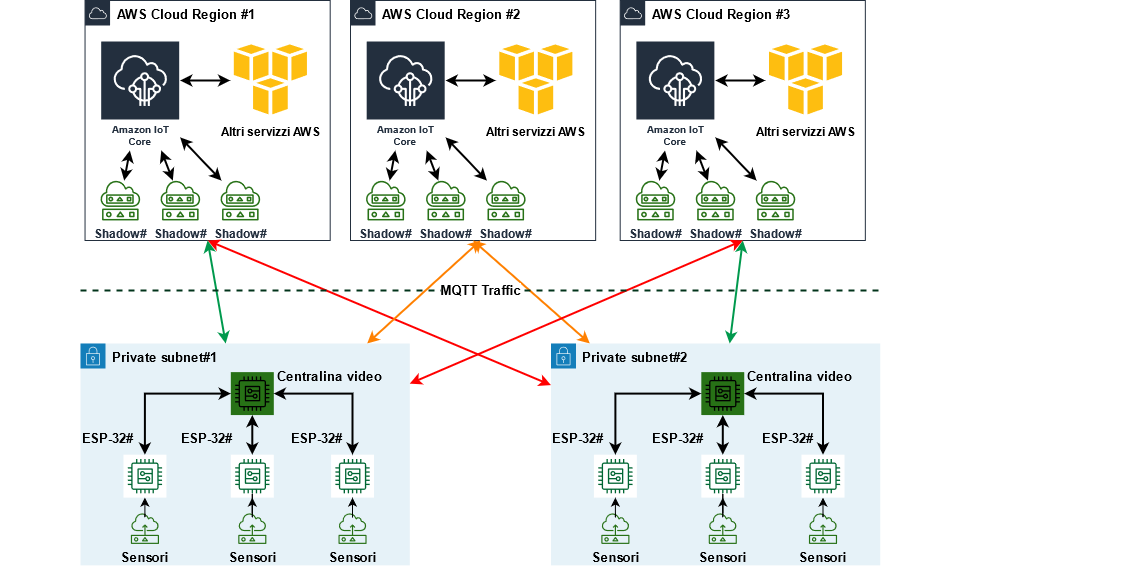
\includegraphics[width=1\textwidth]{DrawIo/ScaledArchitecture.png}
    \end{figure}
 

\section{Analisi Interna}
    I cambiamenti nella rete interna sono relativamente limitati, si suddividono in due parti
    \subsection{Adozione di HW specifico}
    L'utilizzo di Micro-python consente di sviluppare codice per una grande famiglia di micro-controllori. L'ESP-32 è stato scelto anche pensando ad uno sviluppo futuro dato che la sua famiglia presenta varie board che forniscono feature adatte agli ambienti più disparati. Su larga scala è ragionevole pensare che il codice di micro-python opportunamente riadattato consenta la scelta di una qualcunque di queste board alternative fornendo così un'adattabilità in termini di hardware elevata. Ad esempio, vi è la possibilità di integrare ESP che dispongono di tipi di connessione diversi, come l'ESP32-Ethernet-Kit V1.2 e l'ESP32-PICO-KIT-1.
    
    \subsection{Centralina controllo}
    Dato che ogni ESP gestisce un singolo cane e ha una funzione critica, avere un ulteriore livello di controllo dell'ESP locale può aiutare nella preventiva rilevazione dei guasti locali dato che la rete locale è più affidabile ha una minore propensione ai guasti, fornendo alla centralina la possibilità di diagnosticare tramite messaggi interni eventuali guasti, effettuando controlli periodici.
    
    L'integrazione delle funzioni tralasciate nell'applicativo locale realizzato durante questo progetto possono essere introdotte tramite \textbf{Cloud formation} mediante l'utilizzo di \textbf{SAM} (Serverless Application Model). 
    Alcune di queste funzioni sono:
    \begin{itemize}
        \item \textbf{Amazon Cognito:} attualmente il sistema gestisce il salvataggio degli utenti all'interno del DataBase. In un'ottica di deployment su larga scala l'attuale soluzione risulterebbe poco adatta. Un approccio decisamente migliore sarebbe quello di affidare la gestione degli utenti ad Amazon Cognito ed integrarlo con Amazon AWS Amplify.
        \item \textbf{Dynamo DB:} il sistema attuale utilizza due tabelle Dynamo DB, la prima è creata tramite SAM e viene utilizzata per la gestione delle WebSocket, la seconda è creata manualmente e contiene i dati del canile. Dato che la seconda modalità non è applicabile su larga scala, sarebbe necessario automatizzare anche la creazione del database principale, specificando le varie proprietà come lo schema e i valori di throughput.  
        \item \textbf{IoT Core:} è possibile automatizzare il rilascio dei certificati e dei permessi necessari per i dispositivi e aggiungere il relativo dispositivo \textbf{shadow} che mantiene l'ultimo stato conosciuto consentendo così di interrogare il dispositivo anche quando offline.
    \end{itemize}

La libreria UMQTT di Micro-Python consente di utilizzare solo la QoS (Quality of Service) di livello 1 o 0. Attualmente il sistema utilizza QoS di livello 0. Poiché questo applicativo non ha particolari vincoli di velocità per lo scambio dei messaggi è possibile valutare anche l'utilizzo di una QoS superiore. Nel caso in cui si volesse avere la possibilità di avere una QoS di livello 2, che garantisce di ricevere messaggi con certezza, sarà necessario ricorre ad un'alternativa poiché UMQTT supporta fino al livello 1. Sarà inoltre necessario sostituire il broker MQTT di IoT Core con un broker in grado di supportare lvl 2, come ad esempio HiveMQ


\section{Analisi Esterna}
Il database principale gestisce attualmente i dati dei cani, le relative rilevazioni e gli utenti. Questa struttura si è rivelata necessaria poiché ai fini della realizzazione del progetto non vi era la possibilità di sviluppare una parte gestionale in quanto non inerente al corso. Uno sviluppo futuro vede necessaria una rielaborazione del sistema che permetta di effettuare una netta divisione tra la parte gestionale e quella relativa ai dati provenienti dai dispositivi di sensing. Questo porterebbe ad utilizzare il Database attuale solo per immagazzinare le rilevazioni, le quali generano una grande quantità di record. La gestione dei profili dei cani e di quelli degli utenti, andrebbe invece considerata a parte all'interno di un sistema prettamente gestionale. Si potrebbe, ad esempio, utilizzare Amazon Cognito per gestire gli utenti e un DB relazionale per i profili dei cani, il quale porterebbe come vantaggio l'integrità referenziale dei dati e seppur meno performante dovrebbe gestire pochi record.  
    
\section{Analisi complessiva}
    \subsection{Sicurezza}
Nella realizzazione della soluzione attuale non ci si è preoccupati particolarmente della sicurezza. Attualmente le API REST disponibili su API Gateway sono prive di qualunque tipo di autenticazione, questo vale anche per le WEB Socket. Per effettuare il deploy dell'applicativo è necessario autenticare ogni richiesta utilizzando, ad esempio API Gateway Lambda Authorizer. Ciò richiede la scrittura di policy dedicate e maggiormente restrittive rispetto alle attuali full access policy. 

Attualmente i micro-controllori, per autenticarsi presso AWS, utilizzano una chiave privata senza verificare la validità del certificato del server. Questo espone i micro-controllori ad un attacco di tipo \textbf{man in the middle}. Se si volesse fare un utilizzo reale del sistema, questo sarebbe un problema da risolvere in maniera prioritaria.




Se il sistema dovesse essere dispiegato su larga scala si dovrebbe tenere in considerazione il fatto che, a fronte di modifiche a livello di codice, sarebbe pesante dover fare ogni volta il deploy in corso d'opera per testare le funzionalità. Per questo motivo è utile fare in modo che le funzionalità possano essere provate anche in locale, permettendo così di fare il deploy solo quando davvero necessario.
Per abilitare il testing in locale è possibile utilizzare SAM CLI che permette di hostare localmente un'istanza Docker per le chiamale Lambda. 
